% 1962 年全国卷第 8 题：等腰三角形中的内点 D。
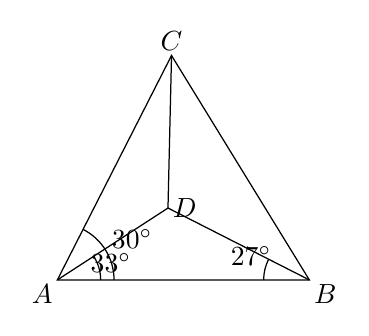
\begin{tikzpicture}[scale=1.0, line width=0.45pt,
  every node/.style={inner sep=1.5pt}]
  \coordinate (A) at (0,0);
  \coordinate (B) at (3.2,0);
  \coordinate (C) at (1.45,2.85);
  \coordinate (D) at (1.405,0.913);
  \draw (A)--(B)--(C)--cycle;
  \draw (A)--(D)--(B);
  \draw (C)--(D);
  \draw (0.55,0) arc (0:33:0.55);
  \draw (0.72,0) arc (0:63:0.72);
  \draw (2.62,0) arc (180:153:0.58);
  \node[anchor=north east] at (A) {$A$};
  \node[anchor=north west] at (B) {$B$};
  \node[anchor=south] at (C) {$C$};
  \node[anchor=west] at (D) {$D$};
  \node at (0.68,0.22) {$33^\circ$};
  \node at (0.95,0.52) {$30^\circ$};
  \node at (2.46,0.3) {$27^\circ$};
\end{tikzpicture}
